\documentclass{TDP003mall}

\usepackage{listings}
\usepackage{float}
\usepackage{array}
\usepackage{color,colortbl}
\usepackage{hyperref}
\usepackage{dirtytalk}
\usepackage{graphicx}

\definecolor{light-gray}{gray}{0.95}
\definecolor{tableshade}{gray}{0.9}

\lstset{
xleftmargin = 0.5cm,
xrightmargin = 0.5cm,
framexleftmargin = 0.5em,
framextopmargin = 0.5em,
framexbottommargin = 0.5em,
frame=single
}

\graphicspath{ {../../images/} }

\newcommand{\version}{Version 1.0}
\author{Mats Eriksson, \url{mater307@student.liu.se}}
\title{Competitive analyze \\ TDP028}
\date{2019-01-04}
\rhead{Mats Eriksson}

\begin{document}
\projectpage
%##############################################################################
\section*{Revisionhistory}
%##############################################################################
\begin{table}[!h]
\begin{tabularx}{\linewidth}{|l|X|l|}
\hline
Ver. & Revision summery & Date \\\hline
1.0 & First draft & 190101 \\\hline
\end{tabularx}
\end{table}


\tableofcontents
\listoffigures
\listoftables
\pagebreak

%##############################################################################
\section{Gather raw data - Different Android applications}
%##############################################################################
The main channel for collecting raw data has been through observing already developed product
in use. This has been in a total active response. Meaning the author has actively tested each
product without any customer nearby. To increase the number of identified needs 3 products has
been selected, which improve the quality of the gather data \cite[chapter 4, p.63]{UlrichEppinger}.
Also for each application each all reviews has been read. Some of them are also been selected for importance
when interpret the raw data into customers need.

From Google play Store three application was chosen.
\begin{itemize}
	\item Actionbound
	\item GPS Quiz
	\item ActiveQuiz
\end{itemize}

 \subsection{Actionbound}
 Actionbound is made by two German programmers and is an application which work like a
 Quiz walk, but without GPS. It has 100000+ downloads and a rate of 3,7 by 790 people.
 It has no review in the Google Play Store. It's possible to make your own quiz (they
 call it bound), through a homepage. The homepage is clean and proper and easy to
 understand. However, an account has to be made to make your bounds.

 Some of the features are:
 \begin{itemize}
  	\item Quiz: You are given three alternative to the question.
		\item Image: Each question has an image.
		\item Points: Each correct answer will reward you with some points.
		\item Compass: The application has a compass. Not sure when to use it.
		\item QR codes: The application can read QR codes by taking a picture.
		\item Take picture: The application can take a picture and store it on a server.
		\item Language: Several languages.
		\item Feedback: Each bound can be rated and review after finished.
		\item Search: It is possible to search for "bounds".
		\item Team: A team of people can share the same phone.
		\item Off-line mode: Each bound can be downloaded.
		\item Indoors/Outdoors: The application could be used both outdoors as well as indoors.
\end{itemize}

First impression of Actionbound are that some features are questionable. The language
only changes on operative functions as buttons, title, etc. The language for the actual game
does not change. Because there is no GPS tracking it does not care if the user actually
is at right location or not. Overall a nice design, big buttons, several layouts and easy
to navigate.
Reading of QR codes and possibility to take pictures make the game more exacting.
It's possible to search for a bound by category, id, new bounds, top ranked and your bounds.
The feedback is comprehensive, which give allot of info when looking for a bound.
The homepage has a good design and it understandable that the application has been on
the market for some time (2012). Even legal information can be clearly shown.

\subsubsection{Screenshot from Actionbound}

\begin{figure}[H]
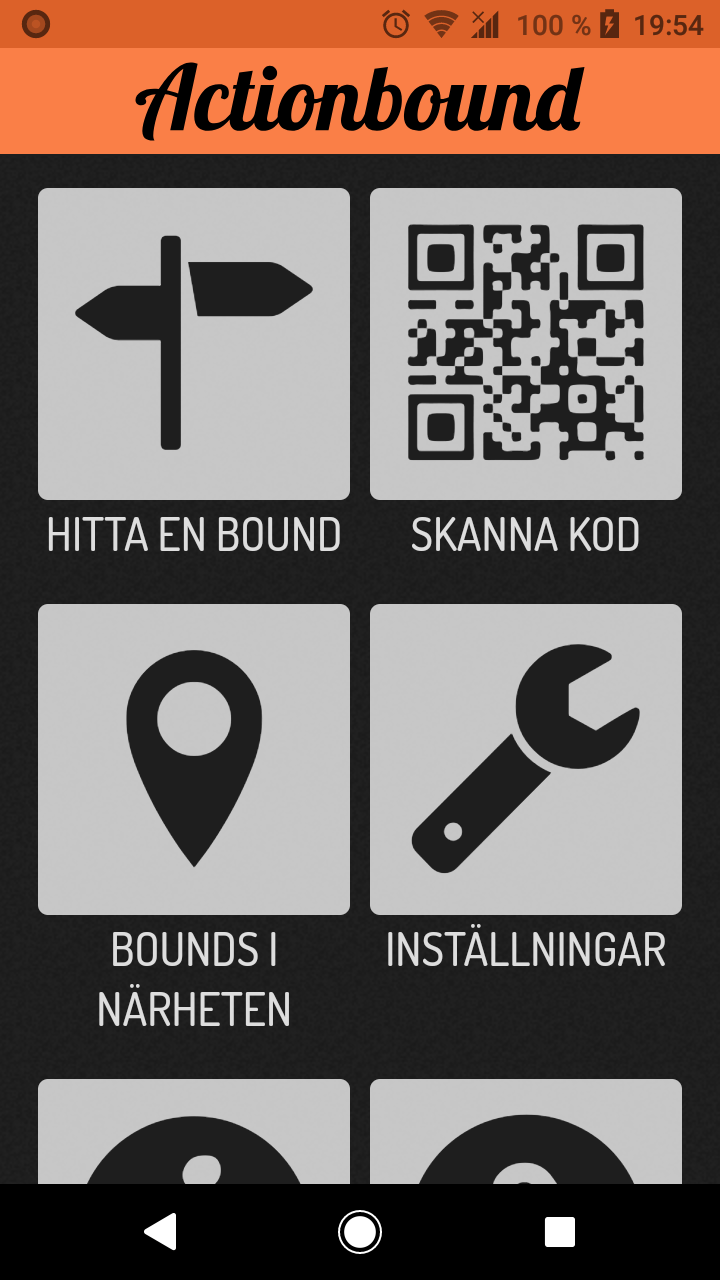
\includegraphics[width=5cm]{pictures/Screenshot_Actionbound1}
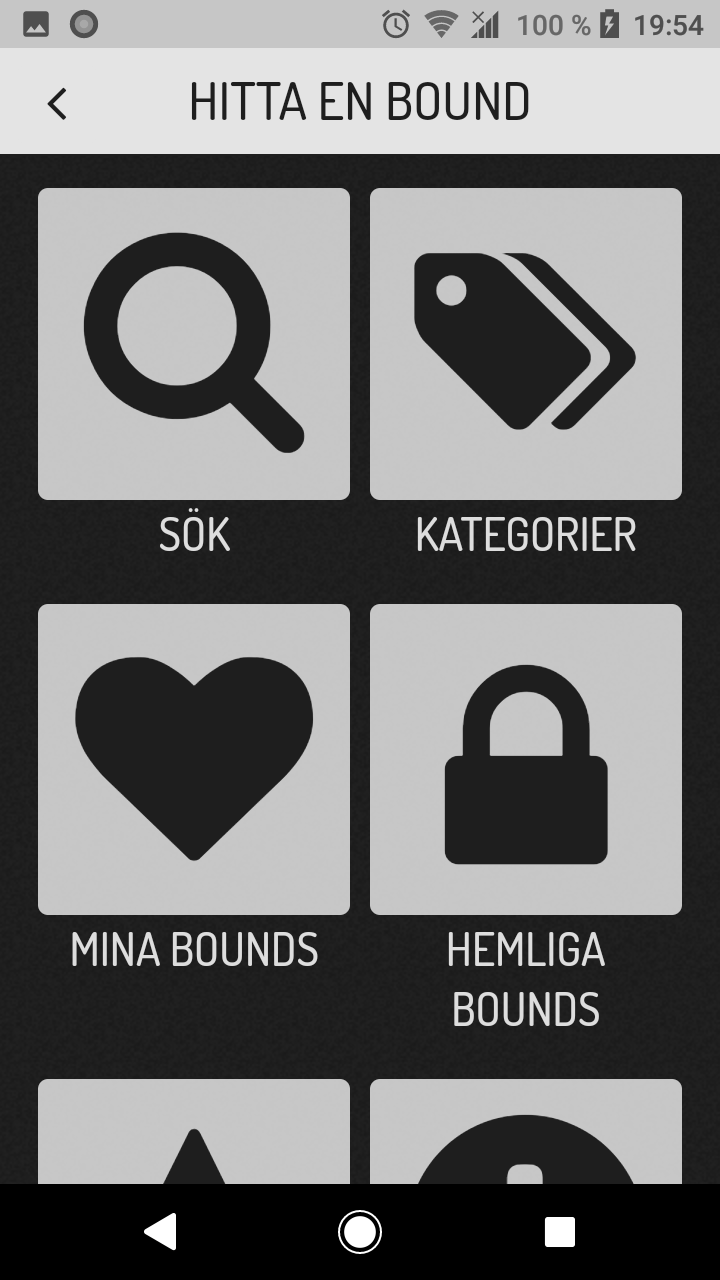
\includegraphics[width=5cm]{pictures/Screenshot_Actionbound2}

\includegraphics[width=5cm]{pictures/Screenshot_Actionbound3}
\centering
\caption{Screenshot of Actionbound}
\end{figure}

\subsection{GPS Quiz}
GPS Quiz is done by a Swedish programmer (Daniel Persson) and is a quiz walk with GPS tracking.
It has around 5000 downloads and a rate of 3.0 by 23 people. It's possible to make your own quiz walk
from a homepage. The homepage is sober and only contains the info you need, which make it easy to navigate.

Some of the feature are:
\begin{itemize}
	\item Continue on an quiz: It is possible to open a quiz which has not being finish and continue on it.
	\item Anonymous walk: The player does not need to login.
	\item Easy access on created quiz: The creator has a separate menu with for its own quiz walks.
	\item Password: Created quiz walks can be protected with a password.
	\item Hidden: Quiz walks which are protected will not be shown in map.
	\item Search: Search for quiz in the area.
	\item Create: Possible to make your own quiz by a homepage.
	\item Image: Each question has an image.
	\item Online result: After finish walk the answers are passed to the server and corrected.
	\item Public result: The result can be read by other.
	\item Google map: The main screen show a map and each position you are going.
\end{itemize}

Outtake of reviews from Google Play Store:
\begin{itemize}
	\item \say{Good precision on the map and pictures show correct. Would be good with a
	function which could remove ongoing path on the map. }
	\item \say{Really need a button to edit the quiz, if you found an error afterwards.}
	\item \say{Need something to detect fake GPS system. }
	\item \say{Can't find any quiz. }
	\item \say{Buttons disappears. Shorter distance then 100 meter for each question. 5-10m
	more realistic. Minor bugs, but good idea and concept. }
\end{itemize}

\subsubsection{First impression}
The main problem with GPS Quiz is that it can't find any quiz walk. The tracking is done
by checking possible quiz walk at that location. Which mean in most cases there is none.
It's almost better that the application would provide a list of possible chooses and the user
could then go there. Right now the user will give up if there is no feedback on where to go.
To make your own quiz walk is easy and only take some minutes. All functions on the homepage
are easy to understand. The user interface on GPS Quiz is the best of the three chosen applications.

\subsubsection{Screenshot from GPS Quiz}

\begin{figure}[H]
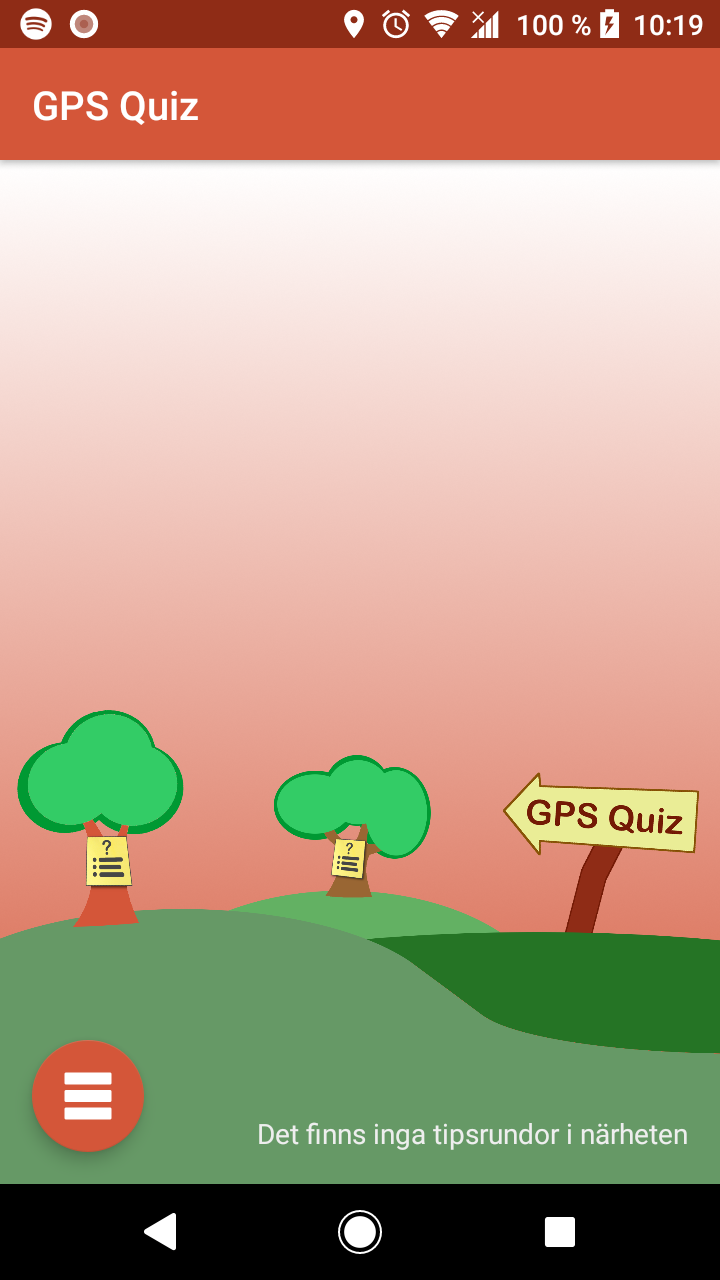
\includegraphics[width=5cm]{pictures/Screenshot_GPS1}
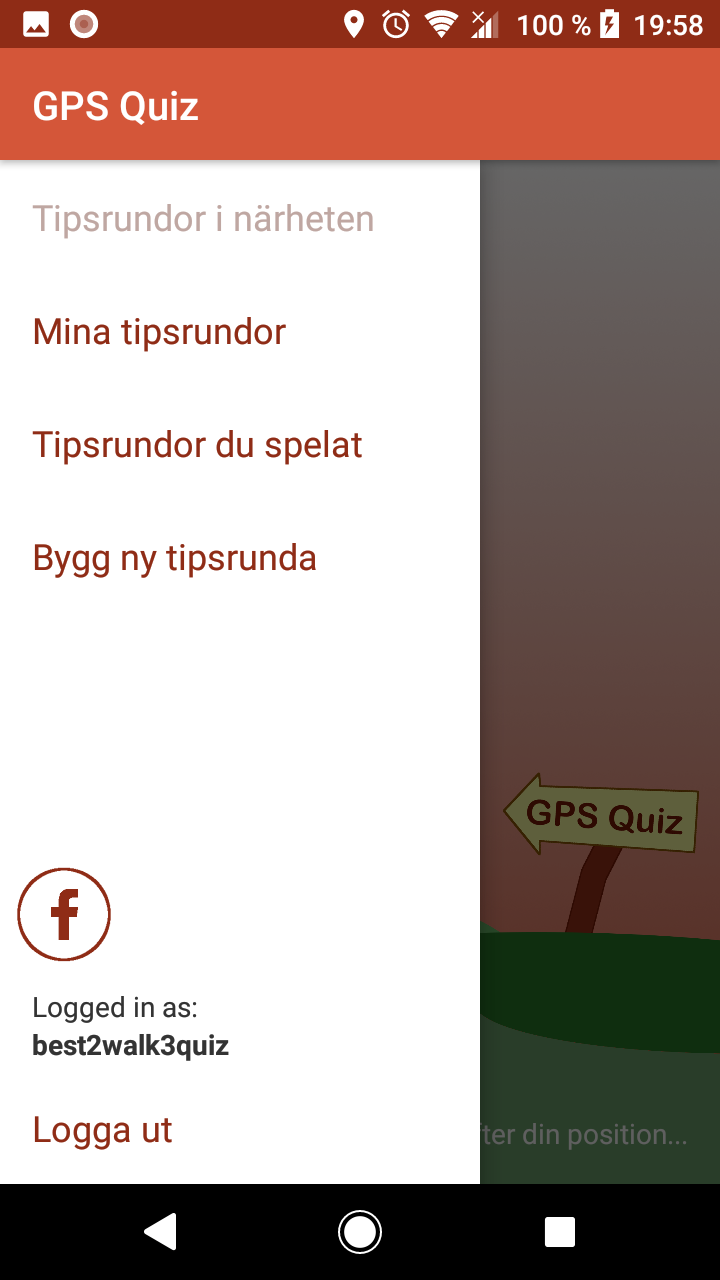
\includegraphics[width=5cm]{pictures/Screenshot_GPS2}
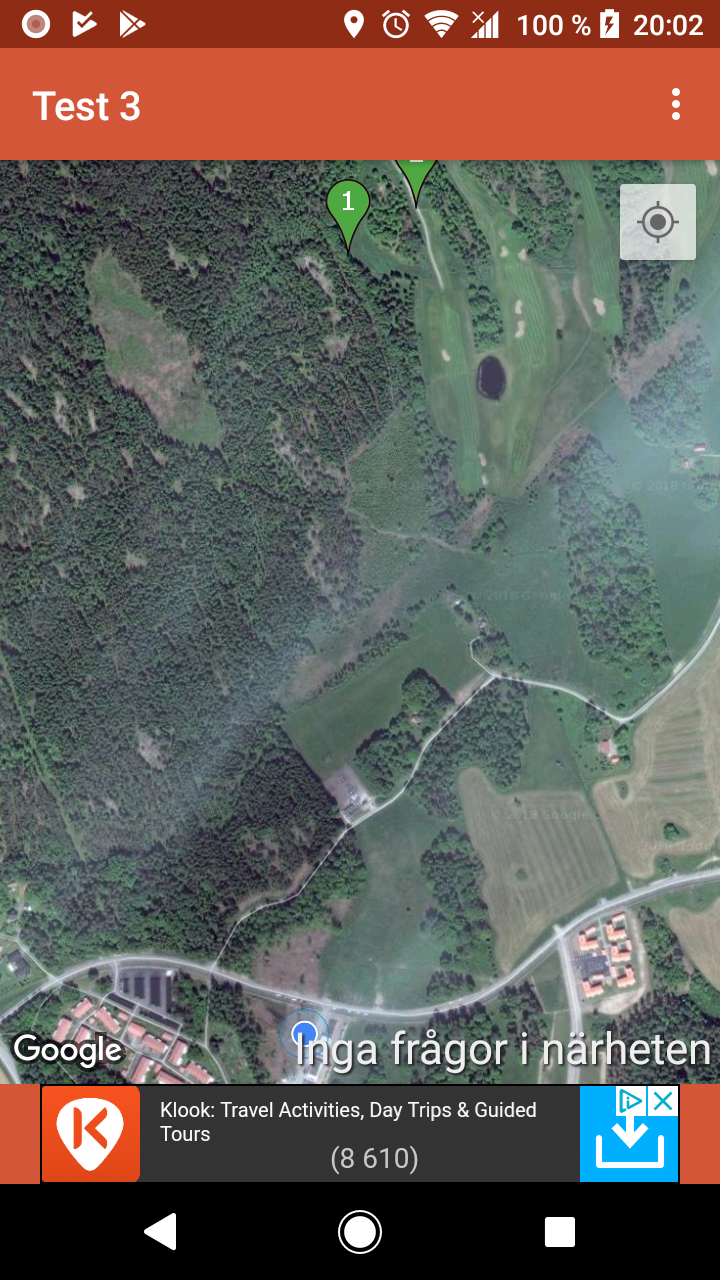
\includegraphics[width=5cm]{pictures/Screenshot_GPS3}
\centering
\caption{Screenshot of GPS Quiz}
\end{figure}

\subsection{ActiveQuiz}
ActiveQuiz is created by a Swedish company called Trilo which usually do applications for
education purpose in age 4-10 years old. This is a quiz walk which uses the GPS system, but only
to detect that the user is actively moving. This means that a new quiz will appear after a certain
amount of meters. According to Google Play Store it has 1000+ downloads and a rate of 4,0 by 16 people.

Some of the features are:
\begin{itemize}
	\item Image: Each question has an image.
	\item Off-line mode: Possible to play without an Internet connection.
	\item Points: The quiz is graded with points.
	\item Highscore: Each quiz has a Highscore list.
	\item Anonymous walk: The player does not need to login.
	\item Max speed: The speed is limited to 16 km/h.
	\item Compete: It's possible to challenge other players.
	\item Search: Possible to select quiz according to category.
	\item Language: Two languages. Swedish and English.
	\item Password: Quiz that you have made can be placed under a password.
	\item Create: Possible to create your own quiz.
\end{itemize}

Outtakes of reviews from Google Play Store:
\begin{itemize}
	\item \say{Need to login everytime. Same questions. I can't send in the result, because the mail
	is not valid}
	\item \say{Nice with pictures to each question.}
	\item \say{Fun to have on your stroll.}
	\item \say{Good combo of movement and digital technology.}
	\item \say{Motion and happiness. Perfect tool for my teaching as a dancer teacher.}
	\item \say{Good tool for teaching of the management group in our company.}
\end{itemize}

\subsubsection{First impression of ActiveQuiz}
The design of the game is very good. However, to move around in all activities is sometimes
not so easy. It's possible to run the game as a guest, even if most of the quiz walks are then
locked. Each quiz walk has a Highscore list adding competitive flavour to the game.
One problem which both GPS quiz and ActiveQuiz is that trackingsystem is very slow with high
lateness. For ActiveQuiz it was hard to even start the game, due to connection lost
from trackingsystem.

\subsubsection{Screenshot from ActiveQuiz}

\begin{figure}[H]
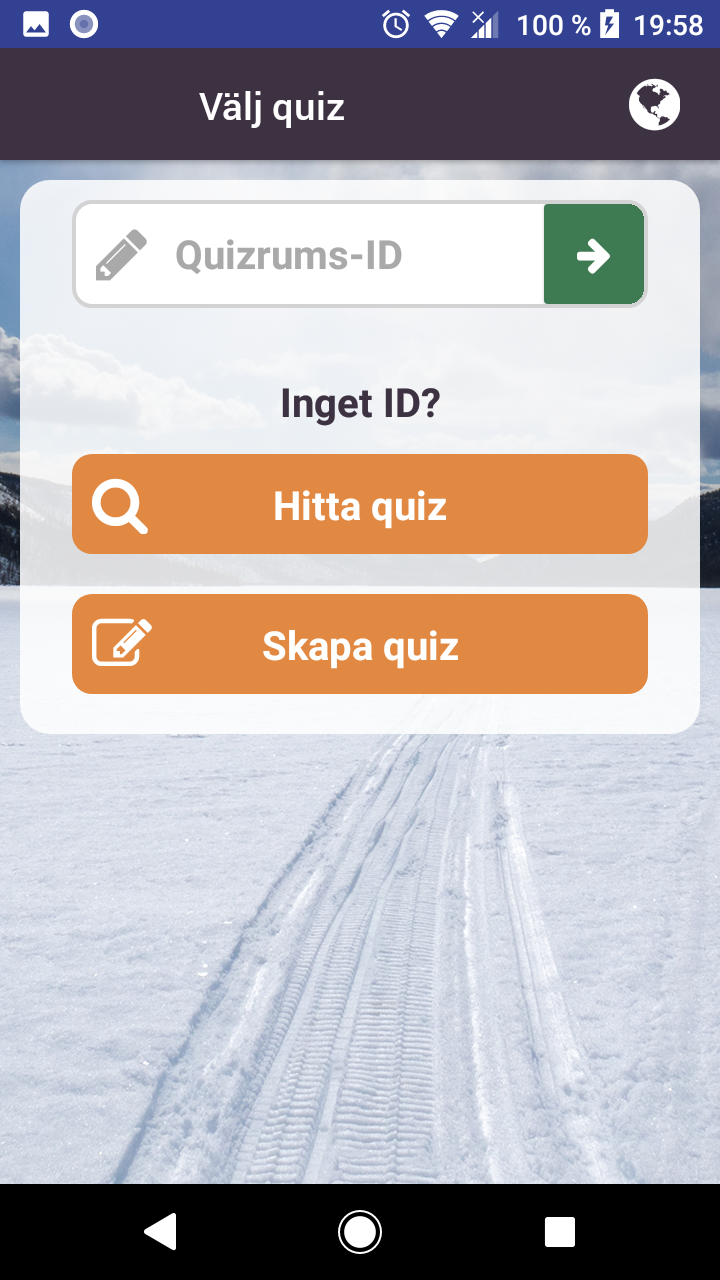
\includegraphics[width=5cm]{pictures/Screenshot_Active1}
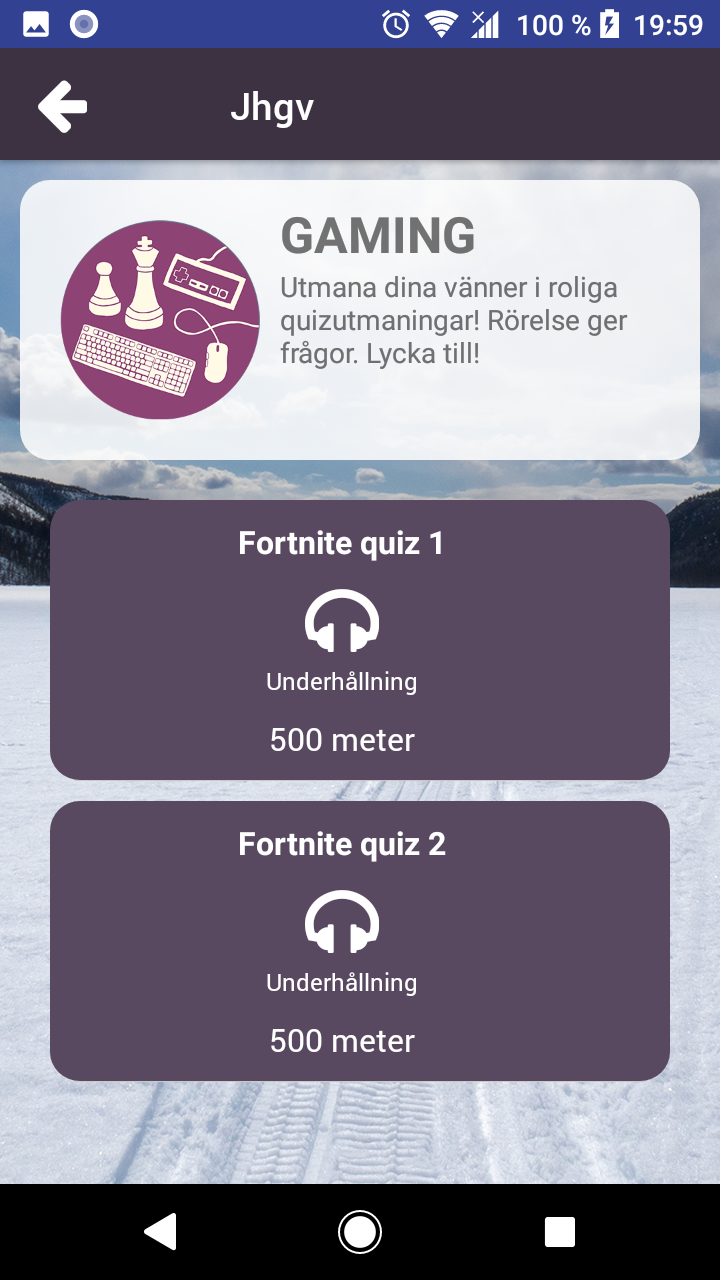
\includegraphics[width=5cm]{pictures/Screenshot_Active2}
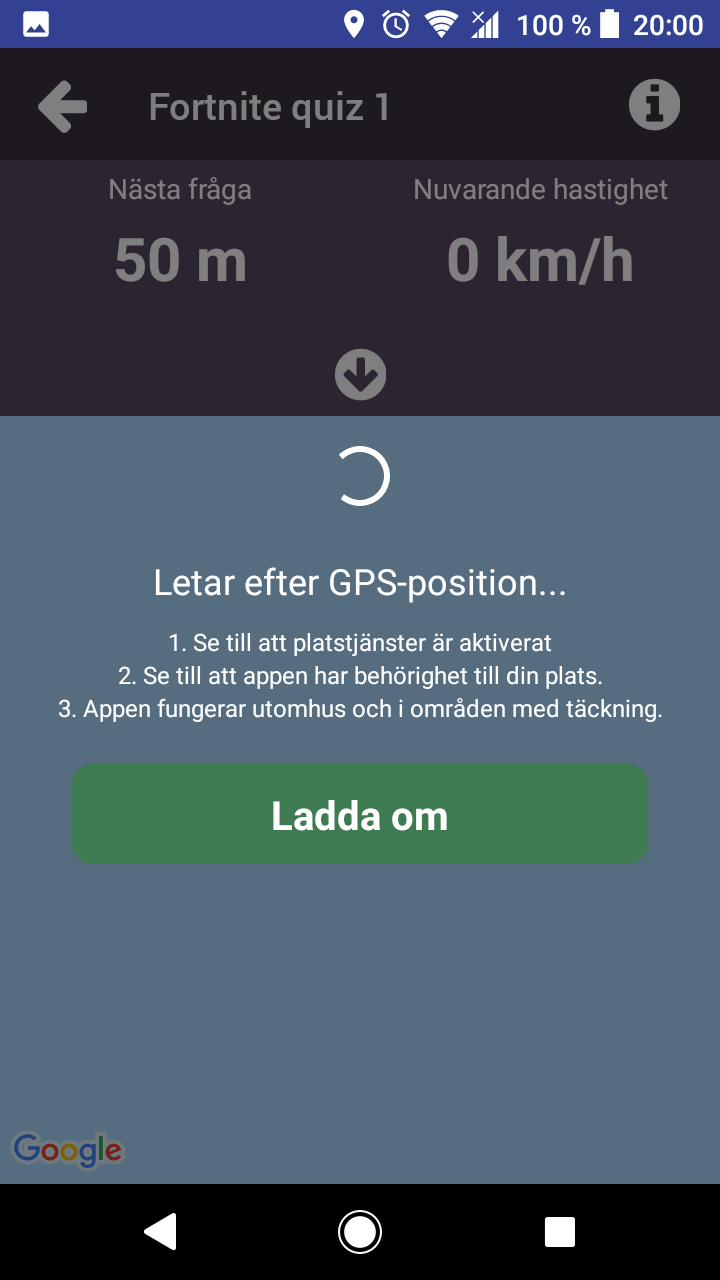
\includegraphics[width=5cm]{pictures/Screenshot_Active3}
\centering
\caption{Screenshot of ActiveQuiz}
\end{figure}

\pagebreak

%##############################################################################
\section{Interpret Raw data in terms of customers needs}
%#############################################################################
Each statement or observation may be translated into any number of customers needs.
Five guidelines has been used as inspiration by converting raw data into customers' needs
\cite[chapter 4, p.~69]{UlrichEppinger}. In this project 10 statements will be done,
which later will be organized into primary needs and secondary needs. The result is rather
surprising, consider my starting specifications. Target specifications probably need to
be changed further down the line of the project.

\begin{itemize}
 	\item Express the need in terms of what the product has to do, not in terms of
	how it might do it.
	\item Express the need as specifically as the raw data
	\item Use positive, not negative, phrasing.
	\item Express the need as an attribute of the product.
	\item Avoid the words must and should.
\end{itemize}

\begin{table}[ht]
\caption{Customer Need Statements}
\centering
\begin{tabular}{l l}
\hline\hline
\# & Need statement \\[0.5ex]
\hline
1 & In game, both picture and question should be received to the user, at each location. \\
2 & The user can create there own game which could be played by friends. \\
3 & The application can run without any Internet connection. \\
4 & The application can give the user a selection of languages to choose from. \\
5 & The user can run the application as anonymous or guest. \\
6 & The application will record the score from the user and compare it to a Highscore list. \\
7 & The user can search for a game, either or in combination of each other, by location, type and category. \\
8 & The quiz created by the user can be protected with password or be hidden from the public. \\
9 & After finishing the game the user can rate the quiz, which can be reviewed by the public. \\
10 & The location system of the application is accurate within a couple of metesr for each quiz. \\ [1ex]
\hline
\end{tabular}
\label{table:CustomerNeedStatements}
\end{table}

\subsection{Organize the Needs into Hierarchy}
In big projects usually around 50-300 statements are created. Because this is a minor exercise,
the amount of times each statement has been reported give me a good view of which statements
could be primary and secondary. The threshold has been placed at middle of the difference, hence 3.
Final result are 4 primary needs and 6 secondary needs.
The specifications which were placed at the beginning of the project does not satisfy these needs
(at least not totally). Target and then final specifications should change, so the application is more
attractive to the customer.

\begin{table}[htb]
\caption{Number of times reported}
\centering
\begin{tabular}{c c}
\hline\hline
Need statement & Number of times reported \\[0.5ex]
\hline
Statement 1 & 5 \\
Statement 2 & 4 \\
Statement 3 & 2 \\
Statement 4 & 1 \\
Statement 5 & 4 \\
Statement 6 & 1 \\
Statement 7 & 3 \\
Statement 8 & 2 \\
Statement 9 & 1 \\
Statement 10 & 2 \\ [1ex]
\hline
\end{tabular}
\label{table:NumberOfTimesReported}
\end{table}

\pagebreak

\subsection{Final tables of customers needs}

\begin{table}[htb]
\caption{Primary needs}
\centering
\begin{tabular}{l}
\hline\hline
Need statement \\[0.5ex]
\hline
In game, both picture and question should be received to the user, at each location. \\
The user can create there own game which could be played by friends. \\
The user can run the application as anonymous or guest. \\
The user can search for a game, either or in combination of each other, by location, type and category. \\ [1ex]
\hline
\end{tabular}
\label{table:PrimaryNeeds}
\end{table}

\begin{table}[htb]
\caption{Secondary needs}
\centering
\begin{tabular}{l}
\hline\hline
Need statement \\[0.5ex]
\hline
The application can run without any Internet connection. \\
The application can give the user a selection of languages to choose from. \\
The application will record the score from the user and compare it to a Highscore list. \\
The quiz created by the user can be protected with password or be hidden from the public. \\
After finishing the game the user can rate the quiz, which can be reviewed by the public. \\
The location system of the application is accurate within a couple of meter for each quiz. \\ [1ex]
\hline
\end{tabular}
\label{table:SecondaryNeeds}
\end{table}

\begin{thebibliography}{9}
\bibitem{UlrichEppinger}
  Karl T. Ulrich, Steven D. Eppinger,
  \textit{Product Design and Development},
  McGraw-Hill Higher Education - ISBN 0-07-229647-X,
  2nd edition,
  2000.
\end{thebibliography}

\end{document}
